%!TEX root = main.tex

\chapter{Results}
This chapter presents results of how our implementation performed
\section{Architecture}
\label{sec:architecture}

\section{In-game performance}

\section{A cognitive cycle}
A cognitive cycle is the a sequence of processes that the cognitive model has to go through from sensing to execution of an action. In LIDA the sequence starts with sensing of the environment, next is understanding, then attention and last is the selection of an action and its execution. These cycles run constantly, and even several of them runs at the same time just in different stages. So when one cycle is finishing brodcasting from the global workspace another can be starting in the sensing phase. 

Following we discribe the complete cognitive cycle that ends with the creation of a new worker unit. 	

\subsection{Sensing}
The first step in the cognitive cycle is sensing. Here sensory-memory samples the environment for new input to the model before low level feature detectors analyzes the input looking for specific features, ideas and meanings. If the feature detector finds something sends excitation to a corresponding feature node in the perceptual associative memory(PAM). Figure \ref{fig:pamtable} shows the table of nodes that we implemented in the project. 
\begin{figure}[h!tb]
\centering
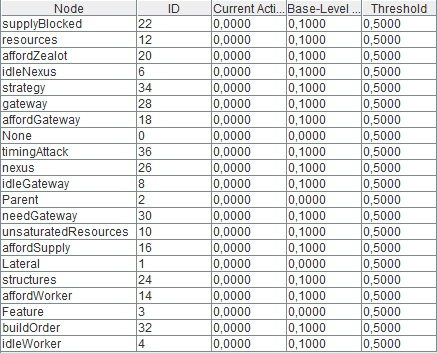
\includegraphics[scale=1.0]{graphics/pam_table.png}
\caption{The PAM table with current activation values}
\label{fig:pamtable}
\end{figure}

\begin{figure}[h!tb]
\centering
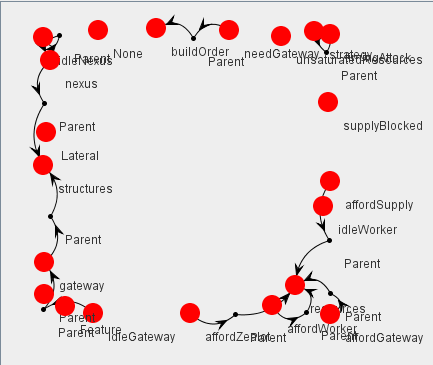
\includegraphics[scale=1.0]{graphics/pam_graph.png}
\caption{Representation of the PAM graph}
\label{fig:pamgraph}
\end{figure}


\subsection{Understanding}
\begin{figure}[h!tb]
\centering
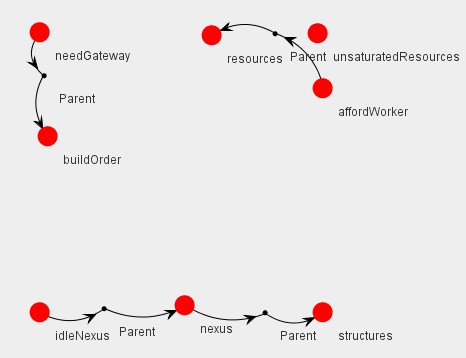
\includegraphics[scale=1.0]{graphics/perceptual_buffer.png}
\caption{The node structure in the perceptual buffer}
\label{fig:perceptbuffer}
\end{figure}

\subsection{Attention}
\begin{figure}[h!tb]
\centering
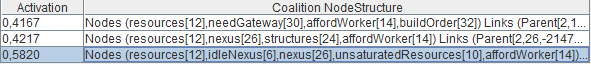
\includegraphics[scale=1.0]{graphics/global_workspace.png}
\caption{Content of the global workspace}
\label{fig:workspace}
\end{figure}

\subsection{Action selection}
\begin{figure}[h!tb]
\centering
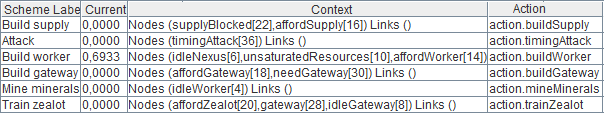
\includegraphics[scale=1.0]{graphics/procedural_memory.png}
\caption{Content of the procedural memory}
\label{fig:proceduralmemory}
\end{figure}

\begin{figure}[h!tb]
\centering
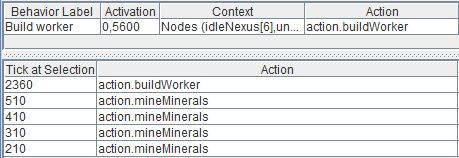
\includegraphics[scale=1.0]{graphics/action_selection.png}
\caption{Content of the action selection module}
\label{fig:actionselection}
\end{figure}
